% $Id$
%


%\usebackgroundtemplate{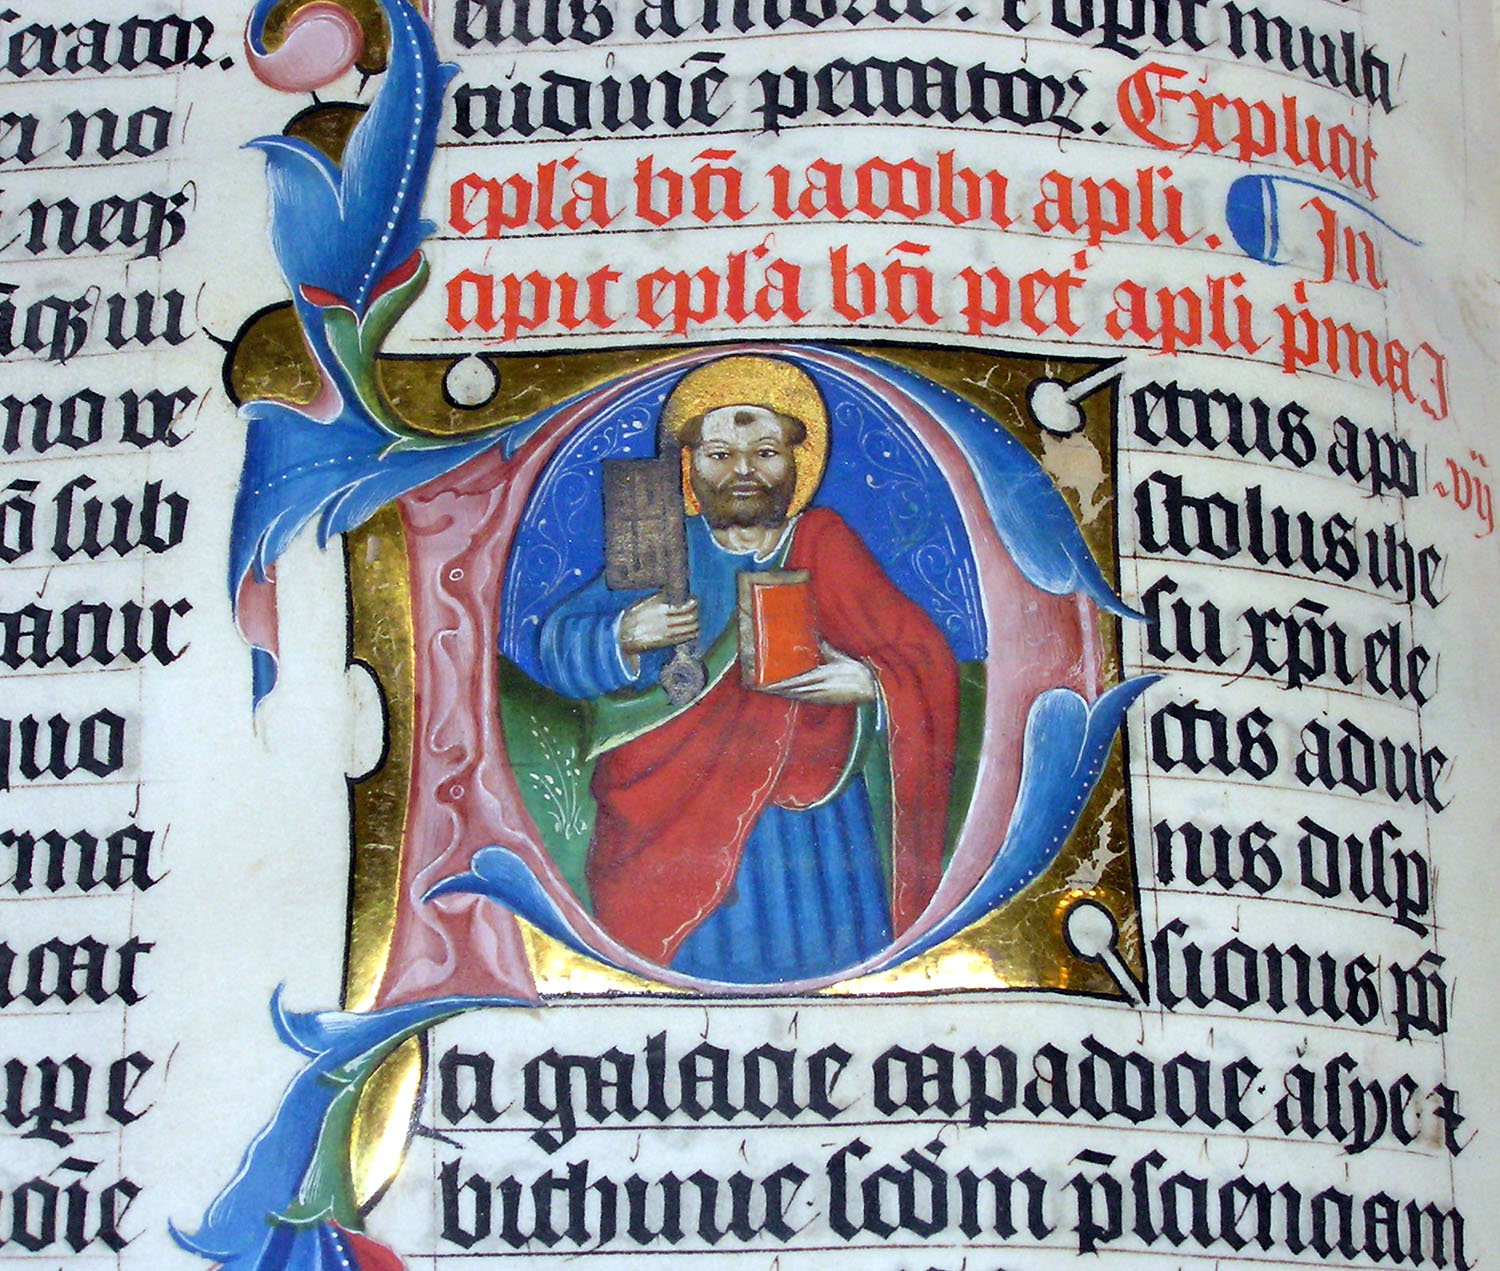
\includegraphics[width=13cm]{figs/biblia}}
%{\bf
%  \textcolor[rgb]{1,1,1}{
    \section{Glosario}
%  }
%}

%\usebackgroundtemplate{}

%%---------------------------------------------------------------

\begin{frame}
\frametitle{Glosarios en comunidad}

{\Large
\begin{itemize}
\item Moodle permite construir glosarios
\item Los alumnos pueden enviar definiciones de t�rminos
\item Las definiciones pueden ser muy completas, incluyendo enlaces, adjuntos...
\item Los alumnos pueden poner comentarios
\item Profesores y alumnos pueden evaluar definiciones
\item Muy interesante para familiazarse con un vocabulario
\end{itemize}
}
\end{frame}




